Over-parameterization is a widely-recognized property of deep neural networks \citep{lowrank1, deep}, which leads to high computational cost and high memory footprint for inference. As a remedy, \emph{network pruning} \citep{obd,obs,han2015learning, nvidia, li2016pruning} has been identified as an effective technique to improve the  efficiency of deep networks for applications with limited computational budget. A typical procedure of network pruning consists of three stages: 1) train a large, over-parameterized model (sometimes there are pretrained models available), 2) prune the trained large model according to a certain criterion, and 3) fine-tune the pruned model to regain the lost performance.

\begin{wrapfigure}{r}[0pt]{0.47\linewidth}
  \begin{center}
  \vspace{-5pt}
    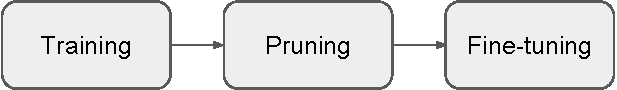
\includegraphics[width=0.47\textwidth]{figures/fig1_pipeline-crop.pdf}
  \end{center}
\caption{A typical three-stage network pruning pipeline.}
    \label{fig1}
    \vspace{-5pt}
\end{wrapfigure}

Generally, there are two common beliefs behind this pruning procedure. First, it is believed that starting with training a large, over-parameterized network is important \citep{luo2017thinet,carreira2018learning}, as it provides a high-performance model (due to stronger representation \& optimization power) from which one can safely remove a set of redundant parameters without significantly hurting the accuracy. Therefore, this is usually believed, and reported to be superior to directly training a smaller network from scratch \citep{li2016pruning,luo2017thinet,he2017channel,nisp} -- a commonly used baseline approach.   
Second, both the pruned architecture \emph{and} its associated weights are believed to be essential for obtaining the final efficient model \citep{han2015learning}. Thus most existing pruning techniques choose to \emph{fine-tune} a pruned model instead of training it from scratch. The preserved weights after pruning are usually considered to be critical, as how to accurately select the set of important weights is a very active research topic in the literature \citep{nvidia,li2016pruning,luo2017thinet, he2017channel, liu2017learning,pfa}.


In this work, we show that both of the beliefs mentioned above are not necessarily true for \emph{structured} pruning methods, which prune at the levels of convolution channels or larger. Based on an extensive empirical evaluation of state-of-the-art pruning algorithms on multiple datasets with multiple network architectures, we make two surprising observations. First, for structured pruning methods with predefined target network architectures (\autoref{auto}), directly training the small target model from random initialization can achieve the same, if not better, performance, as the model obtained from the three-stage pipeline.
In this case, starting with a large model is not necessary and one could instead directly train the target model from scratch.
Second, for structured pruning methods with auto-discovered target networks, training the pruned model from scratch can also achieve comparable or even better performance than fine-tuning. This observation shows that for these pruning methods, what matters more may be the obtained architecture, instead of the preserved weights, despite training the large model is needed to find that target architecture. 
Interestingly, for a \emph{unstructured} pruning method \citep{han2015learning} that prunes individual parameters, we found that training from scratch can mostly achieve comparable accuracy with pruning and fine-tuning on smaller-scale datasets, but fails to do so on the large-scale ImageNet benchmark.
Note that in some cases, if a pretrained large model is already available, pruning and fine-tuning from it can save the training time required to obtain the efficient model.
The contradiction between some of our results and those reported in the literature might be explained by less carefully chosen hyper-parameters, data augmentation schemes and unfair computation budget for evaluating baseline approaches.

\begin{wrapfigure}{r}[0pt]{0.475\linewidth}
    \vspace{-18pt}
  \begin{center}
    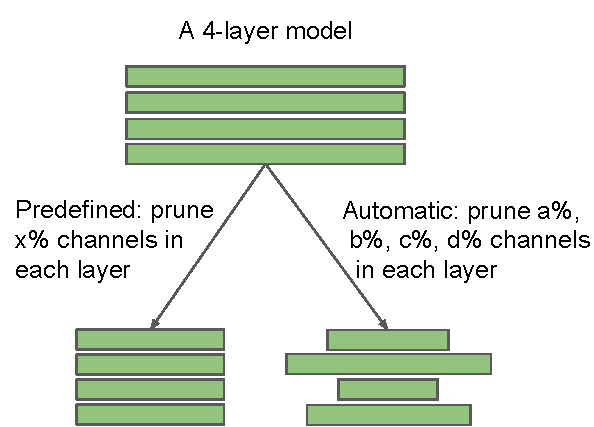
\includegraphics[width=0.45\textwidth]{figures/auto-crop.pdf}
  \end{center}
\caption{Difference between predefined and automatically discovered target architectures, in channel pruning as an example. The pruning ratio $x$ is user-specified, while $a, b, c, d$ are determined by the pruning algorithm. Unstructured sparse pruning can also be viewed as automatic.} 
    \label{auto}
    \vspace{-13pt}

\end{wrapfigure}


Our results advocate a rethinking of existing structured network pruning algorithms. It seems that the over-parameterization during the first-stage training is not as beneficial as previously thought. Also, inheriting weights from a large model is not necessarily optimal, and might trap the pruned model into a bad local minimum, even if the weights are considered ``important'' by the pruning criterion. Instead, our results suggest that the value of automatic structured pruning algorithms sometimes lie in identifying efficient structures and performing implicit architecture search, rather than selecting ``important'' weights. For most structured pruning methods which prune channels/filters, this corresponds to searching the number of channels in each layer. In section 5, we discuss this viewpoint through carefully designed experiments, and show the patterns in the pruned model could provide design guidelines for efficient architectures.

The rest of the paper is organized as follows: in Section 2, we introduce background and some related works on network pruning; in Section 3, we describe our methodology for training the pruned model from scratch; in Section \ref{sec:exp} we experiment on various pruning methods and show our main results for both pruning methods with predefined or automatically discovered target architectures; in Section 5, we discuss the value of automatic pruning methods in searching efficient network architectures; in Section 6 we compare with the recently proposed ``Lottery Ticket Hypothesis'' \citep{lottery}; in Section 7 we discuss some implications and conclude the paper.
